\subsection{Radon-Nikodym and Differentiation}

% **Role:** modern integration and almost-everywhere analysis.
%
% Signed measures, absolute continuity, Radon--Nikodym theorem, Lebesgue differentiation theorem.

This subsection collects the current differentiation-of-measure material. Radon--Nikodym and signed-measure statements can be added here when that source block is expanded.

\begin{figure}[H]
  \centering
  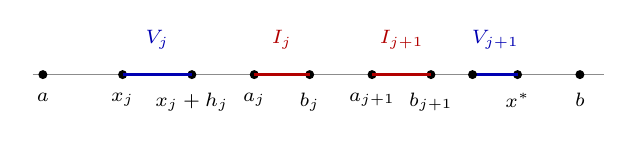
\begin{tikzpicture}[
  scale=0.88,
  every node/.style={font=\scriptsize},
  base/.style={black!45, line width=0.55pt},
  point/.style={circle, fill=black, inner sep=1.15pt},
  controlled/.style={blue!70!black, line width=1.25pt},
  gap/.style={red!70!black, line width=1.15pt},
  labelbox/.style={fill=white, inner sep=1pt}
]
  \draw[base] (-0.15,0) -- (8.1,0);

  \foreach \x/\lab in {
    0/a,
    1.15/x_j,
    2.15/{x_j+h_j},
    3.05/a_j,
    3.85/b_j,
    4.75/a_{j+1},
    5.60/b_{j+1},
    6.85/x^\ast,
    7.75/b
  } {
    \node[point] at (\x,0) {};
    \node[below=3pt] at (\x,0) {$\lab$};
  }

  \draw[controlled] (1.15,0) -- (2.15,0);
  \draw[gap] (3.05,0) -- (3.85,0);
  \draw[gap] (4.75,0) -- (5.60,0);
  \draw[controlled] (6.20,0) -- (6.85,0);
  \node[point] at (6.20,0) {};

  \node[labelbox, text=blue!70!black, above=8pt] at (1.65,0) {$V_j$};
  \node[labelbox, text=red!70!black, above=8pt] at (3.45,0) {$I_j$};
  \node[labelbox, text=red!70!black, above=8pt] at (5.18,0) {$I_{j+1}$};
  \node[labelbox, text=blue!70!black, above=8pt] at (6.53,0) {$V_{j+1}$};
\end{tikzpicture}

  \caption{Interval bookkeeping for absolute continuity.}
  \label{fig:absolute-continuity-interval-decomposition}
\end{figure}

\begin{perspective} \label{per:absolute-continuity-interval-bookkeeping} \hlt{Absolute Continuity as Interval Bookkeeping}\\
If $F(x)=\int_a^x f(t)\,dt$, by absolute continuity, disjoint intervals with small total length force small $F$ total change.\\
\end{perspective}

\begin{figure}[H]
  \centering
  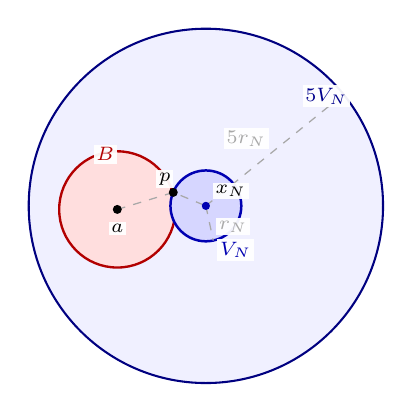
\begin{tikzpicture}[
  scale=0.90,
  every node/.style={font=\scriptsize},
  dilation/.style={draw=blue!50!black, fill=blue!6, line width=0.75pt},
  selected/.style={draw=blue!70!black, fill=blue!16, line width=0.9pt},
  missed/.style={draw=red!70!black, fill=red!13, line width=0.85pt},
  guide/.style={black!34, dashed, line width=0.45pt},
  point/.style={circle, fill=black, inner sep=1.15pt},
  center/.style={circle, fill=blue!70!black, inner sep=1.05pt},
  labelbox/.style={fill=white, fill opacity=0.94, text opacity=1, inner sep=1pt}
]
  \coordinate (x) at (0,0);
  \coordinate (a) at (-1.25,-0.05);
  \coordinate (p) at (-0.46,0.19);

  \draw[dilation] (x) circle (2.50);
  \draw[missed] (a) circle (0.82);
  \draw[selected] (x) circle (0.50);

  \draw[guide] (x) -- ++(39:2.50)
    node[pos=0.48, labelbox, above left=1pt] {$5r_N$};
  \draw[guide] (x) -- ++(-78:0.50)
    node[pos=0.60, labelbox, right=2pt] {$r_N$};
  \draw[guide] (a) -- (p) -- (x);

  \node[point] at (a) {};
  \node[center] at (x) {};
  \node[point] at (p) {};

  \node[labelbox, text=blue!70!black] at (0.42,-0.62) {$V_N$};
  \node[labelbox, text=blue!55!black] at (1.70,1.55) {$5V_N$};
  \node[labelbox, text=red!70!black] at (-1.42,0.73) {$B$};
  \node[labelbox] at (-0.58,0.38) {$p$};
  \node[labelbox] at (-1.25,-0.32) {$a$};
  \node[labelbox] at (0.35,0.21) {$x_N$};
\end{tikzpicture}

  \caption{A comparable missed ball lies inside the fivefold dilation of the selected ball.}
  \label{fig:vitali-fivefold-dilation}
\end{figure}

\begin{perspective} \label{per:vitali-covering-fivefold-control} \hlt{Vitali Covering Control}\\
In a Vitali selection, choose a pairwise disjoint subfamily by decreasing scale. If a candidate ball is not selected, it meets an earlier selected ball of comparable radius, so the fivefold dilation of that selected ball contains it.\\
\hlt{Key Insight}: Disjoint selected balls make measures add, while fixed dilations recover the missed part with bounded overlap cost.
\end{perspective}

\begin{figure}[H]
  \centering
  \begin{tikzpicture}[
  scale=0.86,
  >=Stealth,
  every node/.style={font=\scriptsize},
  axis/.style={->, black!40, line width=0.5pt},
  curve/.style={blue!70!black, line width=0.9pt},
  secant/.style={orange!70!black, line width=0.7pt},
  chosen/.style={orange!85!black, line width=0.9pt},
  guide/.style={black!22, dashed, line width=0.4pt},
  tick/.style={black!50, line width=0.45pt},
  point/.style={circle, fill=black, inner sep=1.15pt},
  labelbox/.style={fill=white, fill opacity=0.94, text opacity=1, inner sep=1pt}
]
  \draw[axis] (-0.35,0) -- (7.85,0) node[right] {$x$};
  \draw[axis] (0,-0.18) -- (0,3.75) node[above] {$y$};

  \coordinate (A) at (0.85,0.62);
  \coordinate (B) at (1.55,1.17);
  \coordinate (C) at (3.20,1.40);
  \coordinate (D) at (4.30,1.86);
  \coordinate (E) at (5.28,2.54);
  \coordinate (F) at (5.98,3.15);

  \draw[curve]
    (0.35,0.43)
    .. controls (0.55,0.48) and (0.70,0.55) .. (A)
    .. controls (1.10,0.72) and (1.22,1.08) .. (B)
    .. controls (2.05,1.34) and (2.70,1.28) .. (C)
    .. controls (3.60,1.48) and (3.94,1.66) .. (D)
    .. controls (4.76,2.08) and (4.96,2.30) .. (E)
    .. controls (5.56,2.73) and (5.64,3.02) .. (F)
    .. controls (6.25,3.35) and (6.95,3.32) .. (7.45,3.40);

  \foreach \p/\q in {A/B,E/F} {
    \draw[secant] (\p) -- (\q);
    \node[point] at (\p) {};
    \node[point] at (\q) {};
  }
  \draw[chosen] (C) -- (D);
  \node[point] at (C) {};
  \node[point] at (D) {};

  \draw[guide] (C) -- (3.20,0);
  \draw[guide] (D) -- (4.30,0);
  \foreach \x in {3.20,4.30} {
    \draw[tick] (\x,0.08) -- (\x,-0.08);
  }
  \node[below=3pt] at (3.20,0) {$x$};
  \node[below=3pt] at (4.30,0) {$x+\frac1n$};

  \node[labelbox, text=blue!70!black] at (2.40,1.58) {$f$};
\end{tikzpicture}

  \caption{$g_n(x)$ is the slope of the short right secant from $x$ to $x+\frac1n$.}
  \label{fig:lebesgue-right-secants}
\end{figure}

\begin{perspective} \label{per:lebesgue-right-secants} \hlt{Right Secants and Differentiation}\\
Right quotients $g_n(x)=n\bigl(f(x+1/n)-f(x)\bigr)$ encode local slope data.\\
\hlt{Key Insight}: Secants turn differentiation into slope estimates.
\end{perspective}
